\section{SeismicSpider}\label{sec:SeismicSpider}

Traditional geophones are mounted in an insulated shock resistive enclosure on a spike. The spikes, varying in length, are inserted into the ground to ensure a firm coupling with the environment. The design of our Seismic Spider prevents full depth insertion of the three inch spikes. 

	To overcome the coupling issue we are using three geophones per station compared to the typical one. Our immediate goals are to compare amplitude and phase response to that of a standard single station.	

\begin{figure} \centering
  {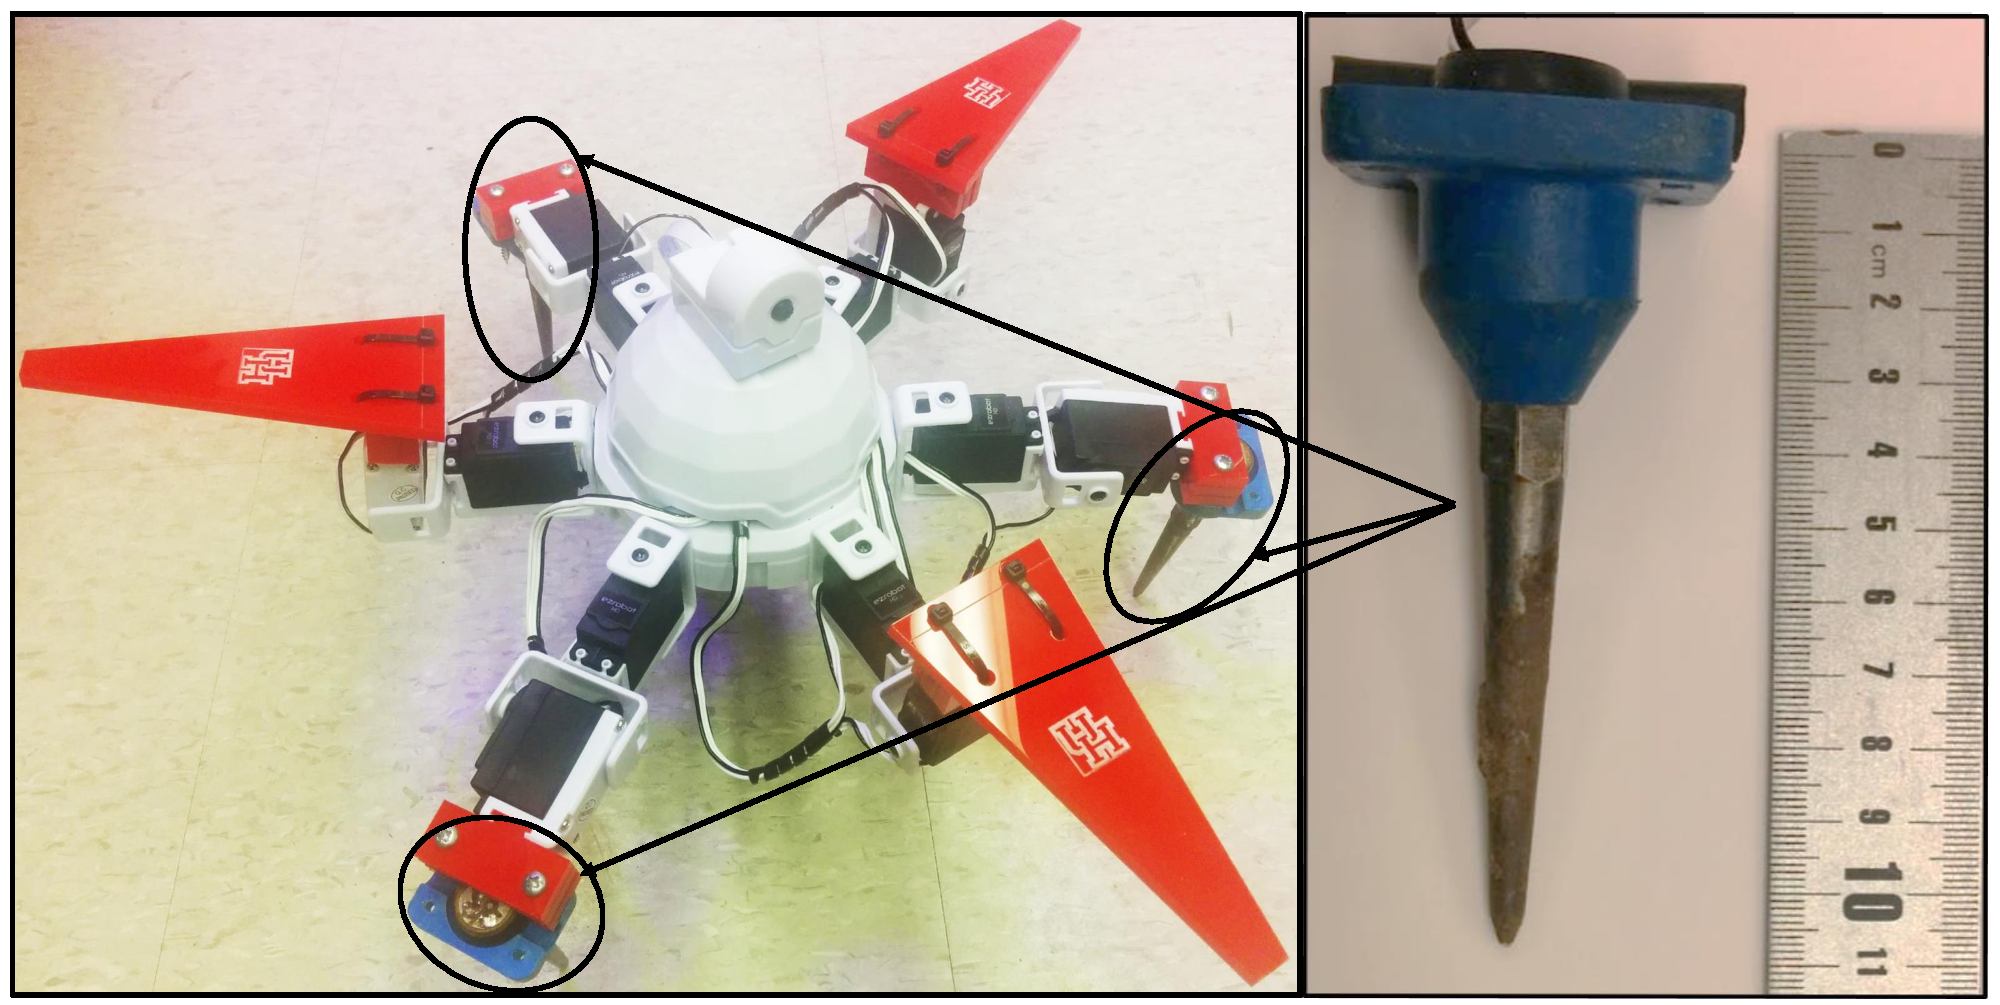
\includegraphics[width=\columnwidth]{Hex_overview.pdf}}
 \caption{The SeismicSpider is a six-legged mobile robot where three legs are replaced by geophones. It senses and records seismic data.} 
 \label{fig:TradvsAutoDrop}
\end{figure}
\subsection{Design}

The Seismic Spider is built from the Six Hexapod kit designed by EZ Robots. Each of the six legs are powered by two 15 kg/cm lever servos. The peg legs were replace by three GS-20DM 14 Hz geophones from Geospace Technologies. The remaining three were designed to match the geophone dimensions and reflect UH school spirit.

 Our initial plan to use three geophones require the spider to raise the three inactive legs while acquiring data. This lack of support caused excessive strain on the three servo motors responsible for holding the spider upright introducing unwanted vibration into the system. We found positioning the geophone legs at 20o to normal enhanced the stability and relieved the excessive stress on the servos. With each planted geophone angled inward superposition creates one vertical geophone. The three geophones were in series.

\subsection{Experiments}
\subsubsection{Exp 1: Accuracy plot}
Hexapod move to desired GPS location  (plot accuracy)\\
\subsubsection{Exp 2: Shot gather comparison}

A line of twenty four geophones, GS-20DM 14 Hz, were laid out at one meter intervals with our inline source seven meters from the nearest geophone. Beginning from the farthest offset of 31 meters we manually aligned the Spider with the corresponding geophone, fired the source, then moved one meter ahead. 

\paragraph{Results}
Data from the shot gather comparison is shown in Fig.~\ref{fig:shotgatherHexpod}.
We found a correlation, unmeasured, with the standard geophones and we more than compensated for loss of amplitude with three geophones, the response was 5 dB greater that the single geophone. The geophone wires proved insufficient to insulate against 60 Hz. Due to the small amount of usable data we were not able to gain meaningful results for phase analysis.   

\begin{figure} \centering
  {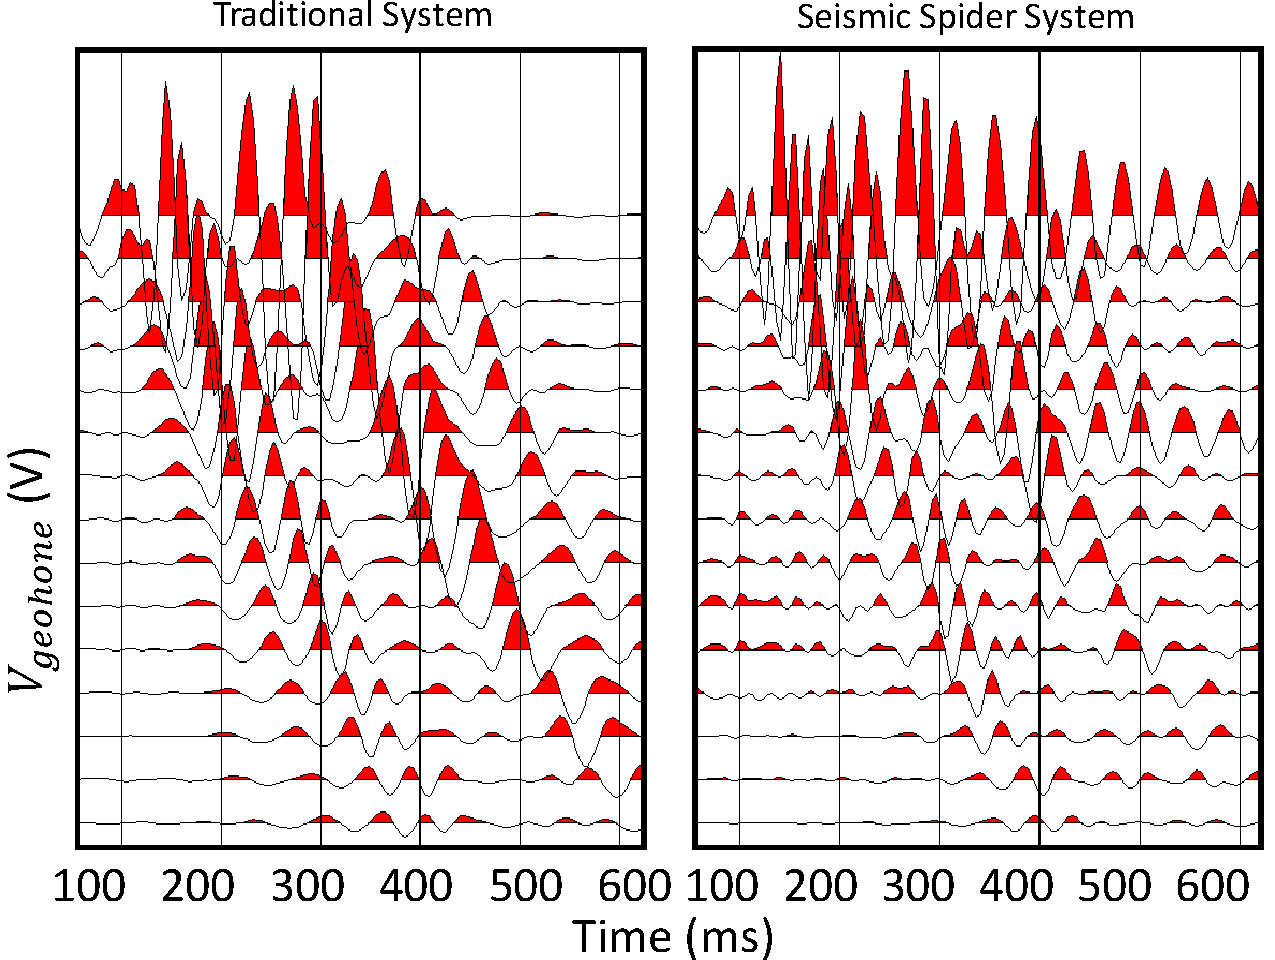
\includegraphics[width=\columnwidth]{shotgather_hex.pdf}}
 \caption{Shot gather comparison of traditional geophones vs. hexapod sensor. 
 \label{fig:shotgatherHexpod}}
\end{figure}


\paragraph{Future work}	we must filter 60 Hz noise, compare adding geophones to all six legs, and design a larger seismic survey to ensure adequate data for phase analysis.   

\subsubsection{Exp 3: Deploying and Retrieving Hexapod}
\todobox{describe piloting the drone for retrieval.  Need image}